\subsection{Outline}

Ola is a full stack developer framework for zero-knowledge applications, the whole framework is shown as \figref{fig:Ola framework}:
\begin{figure}[!ht]
    \centering
    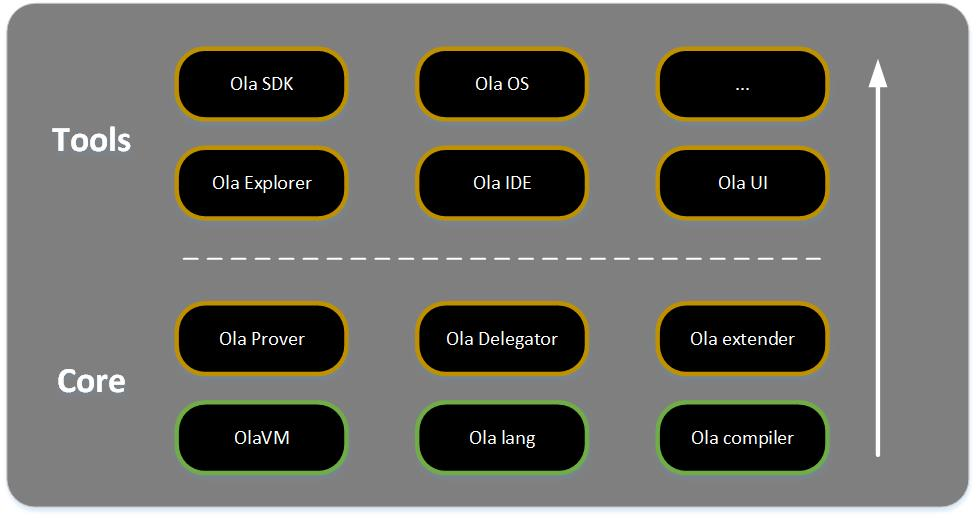
\includegraphics[width=0.6\textwidth]{vm/Ola framework.jpg}
    \caption{Ola framework}
    \label{fig:Ola framework}
\end{figure}

The green borders refers to the modules we have completed implementation, and others stand for the modules we will implement in the future. In the remaining sections of this whitepaper, we will introduce those modules 
as follows:
\begin{itemize}
    \item Section \ref{sec:olavm-a-full-featured-zk-friendly-zkvm} mainly describes the design of Ola's virtual machine, including or zk-friednly design schemes;
    \item Section \ref{sec:ola-lang} mainly describes the design of the customized smart contract language, Ola-lang and the framework of Ola compiler based LLVM;
    \item Section \ref{sec:ola-compiler} mainly describes the design of Ola compiler;
    \item Section \ref{sec:zk-zkvm} mainly describes key points on achieving privacy;
    \item Section \ref{sec:algorithms} mainly describes algorithms used in Ola, including zk and hardware acceleration algorithms;
    \item Section \ref{section:appendix} mainly describes the key features we researched to be supported in the future and our frameworks around that;
    \item Section \ref{sec:glossary} mainly describes some basic notations;
\end{itemize}
